\documentclass[11pt]{beamer}
\usetheme{Malmoe}
\usefonttheme[onlymath]{serif}

\usepackage{graphicx} \usepackage{url} \usepackage{hyperref} \usepackage{caption} \usepackage{amsmath}
\usepackage{amssymb} \usepackage{array} \usepackage{listings} \usepackage{color} \usepackage{textcomp}
\usepackage[utf8]{inputenc} \usepackage{natbib} \usepackage{algorithm} \usepackage{tikz}
\usepackage[noend]{algpseudocode} \usepackage{csquotes} \usepackage{mathtools}

\usetikzlibrary{shapes.geometric, arrows}

\setbeamertemplate{navigation symbols}{}
\setbeamerfont{page number in head/foot}{size=\fontsize{9}{11}}
\setbeamertemplate{footline}[frame number]
\setbeamertemplate{section in toc}{\inserttocsectionnumber.~\inserttocsection}

\author{Glenn Galvizo}
\title{Overview of Solutions to Attitude Determination Problem}
\institute{University of Hawaii at Manoa}

\begin{document}
    \begin{frame}
        \titlepage
    \end{frame}

    \begin{frame}
        \frametitle{Overview}
        \tableofcontents
    \end{frame}

    \section{Background}\label{sec:background}
    \subsection{Story of Procrustes}\label{subsec:storyOfProcrustes}
    \begin{frame}
        \frametitle{Greek Myth: Procrustes}
        \centerline{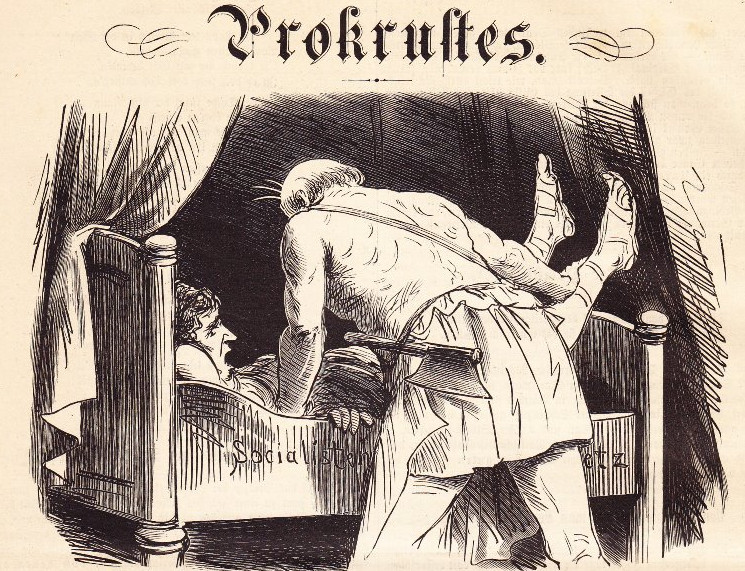
\includegraphics[scale=1.3]{images/procrustes.jpg}}
        % Start with a story.
    \end{frame}

    % Taking a step back. Going to talk about attitude determination.
    \subsection{Spacecraft Attitude Relevancy}\label{subsec:spacecraftAttitudeRelevancy}
    \begin{frame}
        \frametitle{Relevancy: Spacecraft Attitude}
        \begin{definition}
            Attitude determination = process of finding one's \textit{orientation} in space
        \end{definition} \medskip
        \begin{columns}
            \begin{column}{0.5\textwidth}
                \begin{itemize}[<+->]
                    \item Craft uses orientation to: \medskip
                    \begin{enumerate}
                        \item Orient solar panels
                        \item Direct thrusters
                        \item Position payload
                    \end{enumerate} \medskip
                    \item Uses input from: \medskip
                    \begin{enumerate}
                        \item Earth's magnetic field
                        \item Visual position of Sun
                        \item Visual position of stars
                    \end{enumerate}
                \end{itemize}
            \end{column}
            \begin{column}{0.5\textwidth}
                \centering{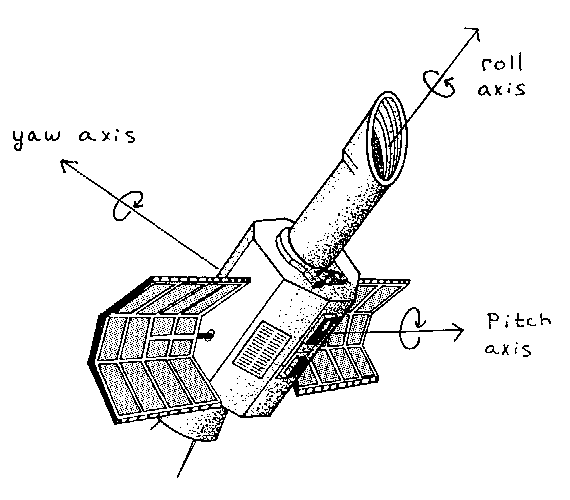
\includegraphics[scale=0.35]{images/spacecraft-attitude.png}}
            \end{column}
        \end{columns}
    \end{frame}

    \begin{frame}
        \frametitle{Attitude Determination}
        \begin{columns}
            \begin{column}{0.5\textwidth}
                \begin{itemize}
                    \item $R \gets$ inertial frame \bigskip
                    \item $B \gets$ body frame \bigskip
                    \item $r_i \gets$ known location in $R$ \bigskip
                    \item $b_i \gets$ observation in $B$
                \end{itemize} \bigskip
            \end{column}
            \begin{column}{0.55\textwidth}
                \centering{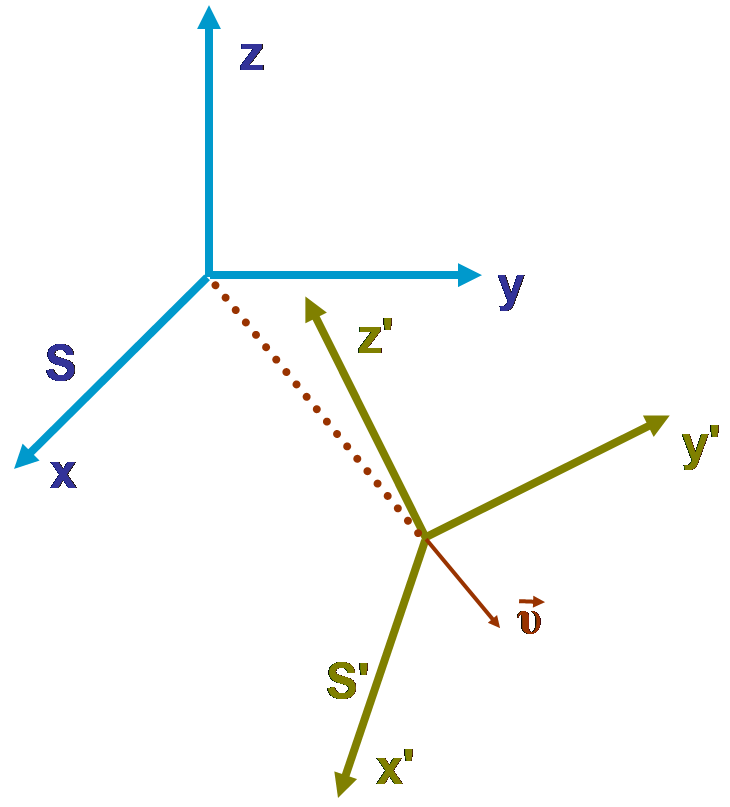
\includegraphics[scale=0.2]{images/inertial-frame.png}}
            \end{column}
        \end{columns} \bigskip
        \centering{\textit{Goal: Find rotation $A$ to take $R$ points to $B$}}
    \end{frame}

    \section{Rotation Representation}\label{sec:rotationRepresentation}
    \begin{frame}
        \begin{center}
            \LARGE{This begs the question\ldots what is $A$?}
        \end{center}
    \end{frame}

    \subsection{Euler Angles}\label{subsec:eulerAngles}
    \begin{frame}
        \frametitle{Euler Angles}
        \begin{definition}
            Euler's Rotation Theorem = Any 3D rotation can be described with three \textit{elementary} rotation angles
        \end{definition}
        \begin{columns}
            \begin{column}{0.5\textwidth}
                \begin{enumerate}
                    \item $\alpha = Z$ rotation \bigskip
                    \item $\beta = Y'$ rotation \\ ($Y$ after (1)) \bigskip
                    \item $\gamma = Z''$ rotation \\ ($Z'$ after (2)) \bigskip
                \end{enumerate}
            \end{column}
            \begin{column}{0.55\textwidth}
                \centering{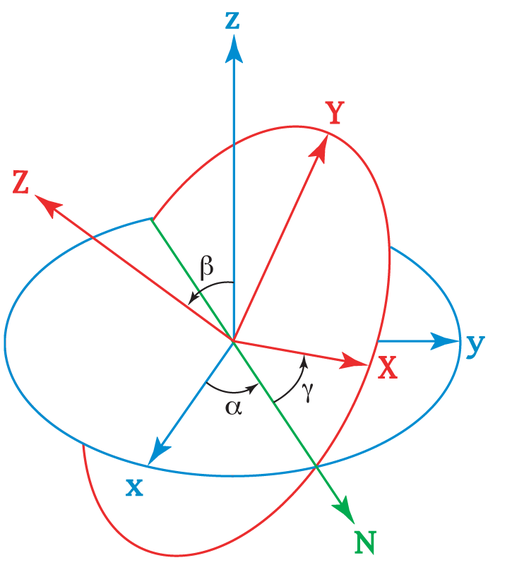
\includegraphics[scale=0.27]{images/euler-angles.png}} \bigskip
            \end{column}
        \end{columns}
    \end{frame}

    \begin{frame}
        \frametitle{Rotation with Euler Angles}\label{subsec:rotationWithEulerAngles}
        \begin{equation}
            \begin{bmatrix}
                r'_1 \\
                r'_2 \\
                r'_3
            \end{bmatrix}
            =
            \begin{bmatrix}
                \cos(\gamma) & \sin(\gamma) & 0 \\
                -\sin(\gamma) & \cos(\gamma) & 0 \\
                0 & 0 & 1
            \end{bmatrix}
            \begin{bmatrix}
                r_1 \\
                r_2 \\
                r_3
            \end{bmatrix}
        \end{equation}
        \begin{equation}
            \begin{bmatrix}
                r''_1 \\
                r''_2 \\
                r''_3 
            \end{bmatrix}
            =
            \begin{bmatrix}
                \cos(\beta) & 0 & -\sin(\beta) \\
                0 & 1 & 0 \\
                \sin(\beta) & 0 & \cos(\beta)
            \end{bmatrix}
            \begin{bmatrix}
                r'_1 \\
                r'_2 \\
                r'_3
            \end{bmatrix}
        \end{equation}
        \begin{equation}
            \begin{bmatrix}
                b_1 \\
                b_2 \\
                b_3
            \end{bmatrix}
            =
            \begin{bmatrix}
                \cos(\alpha) & \sin(\alpha) & 0 \\
                -\sin(\alpha) & \cos(\alpha) & 0 \\
                0 & 0 & 1
            \end{bmatrix}
            \begin{bmatrix}
                r''_1 \\
                r''_2 \\
                r''_3
            \end{bmatrix}
        \end{equation}
    \end{frame}

    \subsection{Rotation Matrices}\label{subsec:rotationMatrices}
    \begin{frame}
        \frametitle{Rotation Matrices}
        \begin{itemize}[<+->]
            \item Original Question: What represents $A$? \medskip
            \item $A$ is a matrix, combining the three equations before. \medskip
            \item We simplify $A$, and represent some rotation as: \medskip
            \begin{equation}
                \begin{bmatrix}
                    b_1 \\
                    b_2 \\
                    b_3
                \end{bmatrix}
                =
                \begin{bmatrix}
                    A_{11} & A_{12} & A_{13} \\
                    A_{21} & A_{22} & A_{33} \\
                    A_{31} & A_{32} & A_{33}
                \end{bmatrix}
                \begin{bmatrix}
                    r_1 \\
                    r_2 \\
                    r_3
                \end{bmatrix}
                = A^{B/R}
                \begin{bmatrix}
                    r_1 \\
                    r_2 \\
                    r_3
                \end{bmatrix}
            \end{equation} \medskip
        \end{itemize}
    \end{frame}

    \subsection{Quaternions}\label{subsec:quaternions}
    \begin{frame}
        \frametitle{Quaternions}
        \begin{itemize}[<+->]
            \item 3D Rotations can be represented as a 3x3 matrix, or a single 4D number \medskip
            \item The relationship between a quaternion $q$ and a direction cosine matrix $A$:
            \begin{equation}
                A =
                \begin{bmatrix}
                    1 - 2(q_2^2 + q_3^2) & 2(q_1 q_2 + q_3 q_4) & 2(q_1 q_3 + q_2 q_4) \\
                    2(q_2 q_1 + q_3 q_4) & 1-2(q_1^2+q_3^2) & 2(q_2 q_3 + q_1 q_4) \\
                    2(q_3 q_1 + q_2 q_4) & 2(q_3 q_2 + q_1 q_4) & 1 - 2(q_1^2+q_2^2)
                \end{bmatrix}
            \end{equation}
            \item Useful for low-power computing as no trigonometry is required
        \end{itemize}
    \end{frame}

    % Interesting note: The (1/2) comes from taking the derivative, to negative the ^2.
    % Least square errors, the weights $v$ are relative to each other (it's a constant factor)
    \section{Wahba's Problem}\label{sec:wahbasProblem}
    \begin{frame}
        \frametitle{Wahba's Problem}
        \begin{definition}
            Wahba's Problem = Finding an \textit{optimal} rotation matrix $A$ to take frame $R$ to $B$, using set of
            observations in both frames
        \end{definition} \medskip

        \begin{itemize}[<+->]
            \item First posed by a mathematician named Grace Wahba \medskip
            \item We seek to minimize the following function:
            \begin{align}
                L(A) &= \frac{1}{2} \sum_i v_i \left\|  b_i - Ar_i \right\|^2 \\
                L(A) &= \lambda_0 - \mathit{tr}\left(AB^T\right)
            \end{align}
            where $\lambda_0 \equiv \sum_i v_i$ and $B \equiv \sum_i v_i b_i r_i^T$. \medskip
            \item \textit{$B$ here is distinct from the spacecraft body frame $B$}
        \end{itemize}
    \end{frame}

    \begin{frame}
        \frametitle{Wahba's Problem}
        \centering{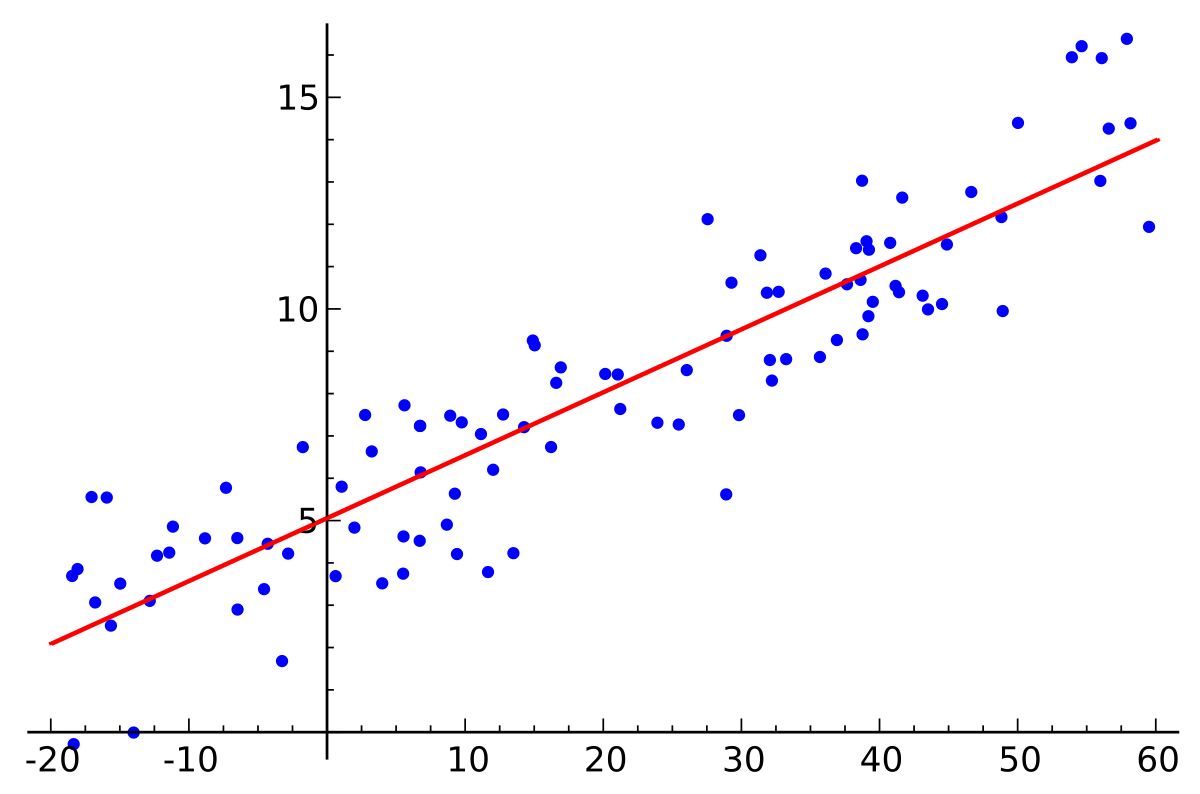
\includegraphics[scale=0.24]{images/linear-regression.png}} \bigskip
        \centering{Like linear regression ($a, b$ terms), but with our 3x3 rotation matrix}
    \end{frame}

    \begin{frame}
        \frametitle{Wahba's Problem}
        \begin{itemize}[<+->]
            \item \textbf{Goal: Minimize $L(A)$}
            \begin{equation*}
                L(A) = \lambda_0 - tr(AB^T)
            \end{equation*}
            where $\lambda_0 \equiv \sum_i v_i$ and $B \equiv \sum_i v_i b_i r_i^T$. \medskip
            \\ How can we do this? \medskip
            \item We cannot minimize $\lambda_0$, so we maximize $tr(AB^T)$\medskip
            \item This can be rewritten as the \textit{orthogonal Procrustes problem}  \medskip
            \begin{itemize}
                \item Added constraint that $\mathit{det} A = 1$ \medskip
            \end{itemize}
            \item Known approaches: SVD, Q Method, TRIAD \medskip
        \end{itemize}
    \end{frame}

    % Note: we cannot change matrices V and U here, but we can change
    \section{Solutions to Wahba's Problem}\label{sec:wahbasProblemSolutions}
    \subsection{SVD Method}\label{subsec:svdMethod}
    \begin{frame}
        \frametitle{SVD Method (Singular Value Decomposition)}
        \begin{itemize}[<+->]
            \item  = factorization of some matrix into three different matrices \medskip
            \item $B$ can be factored into:
            \begin{equation}
                B = U \Sigma V^T = U diag \left[ \Sigma_{11} \ \Sigma_{22} \ \Sigma_{33} \right] V^T
            \end{equation}
            where $U$ and $V$ are orthogonal, and $\Sigma_{11} \geq \Sigma_{22} \geq \Sigma_{33} \geq 0$ \medskip
            \item $\Sigma$ represents diagonal matrix containing square roots of eigenvalues from $U$ or $V$ in
            descending order \medskip
            \item The optimal rotation is defined as:
            \begin{equation}
                A_{opt} = U diag \left[ 1 \ 1 \ (\mathit{det} U)(\mathit{det} V) \right] V^T
            \end{equation}
        \end{itemize}
    \end{frame}

    \subsection{Q Method}\label{subsec:qMethod}
    \begin{frame}
        \frametitle{Q Method}
        \begin{itemize}[<+->]
            \item = \textit{Davenport's Q Method} \medskip
            \item Parameterized rotation matrix with a unit quaternion \medskip
            \item Rewrite trace maximization as:
            \begin{equation}
                \mathit{tr}\left(AB^T \right) = q^T K q
            \end{equation}
            where $K$ is symmetric and traceless:
            \begin{equation*}
                K \equiv
                \begin{bmatrix}
                    S - I \mathit{tr}\left(B\right) & z \\
                    z^T & \mathit{tr}\left(B\right)
                \end{bmatrix}
            \end{equation*}
            \begin{equation*}
                \text{with } S = B + B^T \text{ and } z \equiv
                \begin{bmatrix}
                    B_{23} - B_{32} \\
                    B_{31} - B_{13} \\
                    B_{12} - B_{21}
                \end{bmatrix}
                =
                \sum_i a_i b_i \times r_i
            \end{equation*}
        \end{itemize}
    \end{frame}

    \begin{frame}
        \frametitle{Q Method}
        \begin{itemize}[<+->]
            \item We still want to maximize $q^T K q$ \medskip
            \item We cannot change $K$, so we construct the following:
            \begin{equation}
                K q_{opt} \equiv \lambda_{max} q_{opt}
            \end{equation}
            \item This is the symmetric eigenvalue problem \medskip
            \item QUEST Method specifies how to find $\lambda_{max}$ efficiently
        \end{itemize}
    \end{frame}

    \subsection{TRIAD Method}\label{subsec:triadMethod}
    \begin{frame}
        \frametitle{TRIAD Method}
        \begin{itemize}[<+->]
            \item Introduces a third frame (hence the name) \medskip
            \item Doesn't try to minimize $L(A)$, only uses $b_1, b_2, r_1, r_2$ \medskip
            \item Treats one observation $b_1, r_1$ as \textbf{true}
            \begin{align}
                t_{1b} &= b_1 \\
                t_{1r} &= r_1
            \end{align}
            \item Second vector $t_2$ is perpendicular to two observations, and normalized:
            \begin{align}
                t_{2b} &= \frac{b_1 \times b_2}{\lvert b_1 \times b_2 \rvert} \\
                t_{2r} &= \frac{r_1 \times r_2}{\lvert r_1 \times r_2 \rvert}
            \end{align}
        \end{itemize}
    \end{frame}

    \begin{frame}
        \frametitle{TRIAD Method}
        \begin{itemize}[<+->]
            \item Third vector completes the TRIAD:
            \begin{align}
                t_{3b} &= t_{1b} \times t_{2b} \\
                t_{3r} &= t_{1r} \times t_{2r}
            \end{align}
            \item Our rotation matrix becomes:
            \begin{equation}
                R =
                \begin{bmatrix}
                    t_{1b} & t_{2b} & t_{3b}
                \end{bmatrix}
                \begin{bmatrix}
                    t_{1r} & t_{2r} & t_{3r}
                \end{bmatrix}^T
            \end{equation}
            \item First term = $B$ to the TRIAD frame \medskip
            \item Second term = $R$ to the TRIAD frame
        \end{itemize}
    \end{frame}

    \section{}

    \section*{}
    \begin{frame}
        \frametitle{Conclusion}
        \begin{enumerate}[<+->]
            \item 3D rotations are 3x3 matrices, or a single 4D vector \medskip
            \item Wahba's problem aims to minimize some function to find a rotation \medskip
            \item SVD works, but is computationally expensive \medskip
            \item Q Method (solved by QUEST) is most widely used \medskip
            \item TRIAD Method is simplest, but discards a lot of information
        \end{enumerate}
    \end{frame}

    \begin{frame}
        \centering{\huge{Questions?}}
    \end{frame}
\end{document}
